\section{Image preprocessing}
\label{sec:cli:input:image:preprocessing}


\begin{figure}
\begin{center}
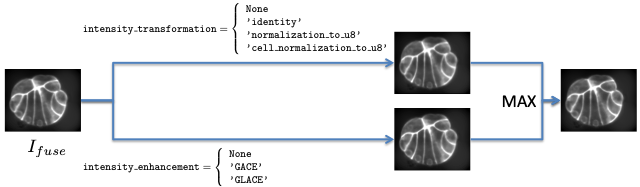
\includegraphics[height=50mm]{figures/build-input-segmentation.png}
\end{center}
\caption{\label{fig:cli:input:image:preprocessing}
The input for segmentation (ie $h$-minima computation, seeded watershed) is built from (eventually) two images derived from the fusion image.}
\end{figure}


The segmentation of membranes images is based on a seeded watershed. Seeds are computed from either one single regional minima image (segmentation of the first time point, see section \ref{sec:cli:mars}) or several ones (segmentation by propagation of the other time points, see section \ref{sec:cli:astec}).


The regional minima operation, as well as the watershed operation, are conducted on the pre-processed version of the fused image. More precisely, the fused image may undergo two kinds of pre-processing, one denoted \option{intensity\_transformation} (and transform the image values based on its histogram) and the other \option{intensity\_enhancement} (and transform the image based on a membrane dedicated process). The image used for segmentation is the fusion (by the maximum) of these two pre-processing results (see figure \ref{fig:cli:input:image:preprocessing}).

If the fused image is transformed before being segmented, the transformed image is named \texttt{<EN>\_fuse\_t<timepoint>\_membrane.inr} and stored in the directory \texttt{SEG/SEG\_<EXP\_SEG>/RECONSTRUCTION/} if the value of the variable \option{keep\_reconstruction} is set to \texttt{True}.

Note that specifying 
\begin{verbatim}
intensity_transformation = 'identity'
intensity_enhancement = None
\end{verbatim}
in the parameter file comes to use the unprocessed fused image as input image for the segmentation.


\subsection{Histogram based image value transformation}
\label{sec:cli:input:image:preprocessing:histogram}

The option \option{intensity\_transformation} can be set to one out the three (segmentation of the first time point, see section \ref{sec:cli:mars}) or four (segmentation by propagation of the other time points, see section \ref{sec:cli:astec}) values.
\begin{itemize}
\itemsep -0.5ex
\item \texttt{None}: this pre-processing channel is not used, meaning that only the membrane dedicated process will produce the input for the segmentation.
\item \texttt{'identity'}: there is no transformation of the fused image.
\item \texttt{'normalization\_to\_u8'}: input images are usually encoded on 2 bytes. However, it is of some interest to have input images of similar intensity distribution, so the segmentation parameters (eg the $h$'s for the regional minima computation) do not have to be tuned independently for each image or sequence.

This choice casts the input image on a one-byte image (ie into the value range $[0, 255]$) 
by linearly mapping the fused image values from $[I_{min}, I_{max}]$ to $[0, 255]$. $I_{min}$ and $I_{max}$ correspond respectively to the 1\% and to the 99\% percentiles of the fused image cumulative histogram. This allows to perform a robust normalization into $[0, 255]$ without being affected by extremely low or high intensity values.
Values below $I_{min}$ are set to $0$ while values above $I_{max}$ are set to $255$.

The percentiles used for the casting can be tuned by the means of two variables
\begin{verbatim}
normalization_min_percentile = 0.01
normalization_max_percentile = 0.99
\end{verbatim}

\item \texttt{'cell\_normalization\_to\_u8'}: this choice can only be used for the segmentation propagation (see section \ref{sec:cli:astec}). It has been developed (and kept) for historical reasons but has not proven to be useful yet. 
 
The segmentation (the image of cell labels) at time point $t$, $S^{\star}_t$, is first deformed onto the image at time $t+1$ thanks to the transformation $\mathcal{T}_{t \leftarrow t+1}$ from the image $I^{t+1}_{fuse}$ at time $t+1$ towards to image $I^{t}_{fuse}$ at time $t$ (this transformation is computed with the fused images). The deformed segmentation can be denoted by $S^{\star}_t \circ \mathcal{T}_{t \leftarrow t+1}$. 
According that the co-registration of the image $I^{t+1}_{fuse}$ and $I^{t}_{fuse}$ is successful, this deformed segmentation is an estimated segmentation (without any cell division) of $I^{t+1}_{fuse}$. 

Instead of computing one histogram for the whole image as in the \texttt{'normalization\_to\_u8'}, and thus having one $I_{min}$ and one $I_{max}$ value for the whole image, histogram are here computed on a cell basis, and a couple $(I_{min}, I_{max})$ is computed for each label of $S^{\star}_t \circ \mathcal{T}_{t \leftarrow t+1}$, yielding images of values $I_{min}$ and $I_{max}$. Since this induces discontinuities at cell borders, these two images are smoothed (with a Gaussian filter of standard deviation \option{cell\_normalization\_sigma} before casting into $[0, 255]$.

For each cell, different histogram can be used for the computation of $I_{min}$ and $I_{max}$.
\begin{itemize}
\itemsep -0.5ex
\item \option{cell\_normalization\_max\_method} sets the cell area where to compute the histogram for the $I_{max}$ value, while
\item \option{cell\_normalization\_min\_method} sets the cell area where to compute the histogram for the $I_{min}$ value.
\end{itemize}

Cell areas can be defined as
\begin{itemize}
\itemsep -0.5ex
\item \option{cell}: all the values of $I^{t+1}_{fuse}$ below the aimed cell defined in $S^{\star}_t \circ \mathcal{T}_{t \leftarrow t+1}$ are used for the histogram computation, 
\item \option{cellborder}: only the values of $I^{t+1}_{fuse}$ at the aimed cell border defined in $S^{\star}_t \circ \mathcal{T}_{t \leftarrow t+1}$ are used for the histogram computation, and 
\item \option{cellinterior}: all the value of $I^{t+1}_{fuse}$ in the aimed cell interior (the border is excluded) defined in $S^{\star}_t \circ \mathcal{T}_{t \leftarrow t+1}$ are used for the histogram computation.
\end{itemize}

Default values are 
\begin{verbatim}
cell_normalization_max_method = 'cellborder'
cell_normalization_min_method = 'cellinterior'
\end{verbatim}
meaning that $I_{max}$'s are computed at the cells' borders while $I_{min}$'s are computed in the cells' interiors. 
\end{itemize}


\subsection{Membrane dedicated enhancement}
\label{sec:cli:input:image:preprocessing:membrane}

The option \option{intensity\_transformation} can be set to one out the two (segmentation of the first time point, see section \ref{sec:cli:mars}) or three (segmentation by propagation of the other time points, see section \ref{sec:cli:astec}) values.

\begin{itemize}
\itemsep -0.5ex
\item \texttt{None}: this pre-processing channel is not used, meaning that only the histogram based image value transformation will produce the input for the segmentation.
\item \texttt{'GACE'} stands for \textit{Global Automated Cell Extractor}. This is the method described in \cite{michelin:hal-00915000,michelin:tel-01451608}.
\item \texttt{'GLACE'} stands for \textit{Grouped Local Automated Cell Extractor}. It differs from one step from \texttt{GACE}: the threshold of extrema image is not computed globally (as in \texttt{GACE}), but one threshold is computed per cell of $S^{\star}_{t-1} \circ \mathcal{T}_{t-1 \leftarrow t}$, from the extrema values of the cell bounding box.
\end{itemize}

\texttt{GACE} and \texttt{GLACE} consist both of the following steps.

\begin{enumerate}
\itemsep -0.5ex

\item Membrane dedicated response computation. The Hessian is computed by convolution with the second derivatives of a Gaussian kernel (whose standard  deviation is given by \option{mars\_sigma\_membrane}). The analysis of eigenvalues and vectors of the Hessian matrix allows to recognize the normal direction of an eventual membrane. A response is then computed based on a contour detector in the membrane normal direction.

\item Directional extrema extraction. Extrema of the response in the direction of the membrane normal are extracted. It yields a valued image of membrane centerplanes.

\item \label{it:gace:threshold} Direction dependent automated thresholding.

It has been observed that the membrane contrast depends on the membrane orientation with respect to the microscope apparatus. Directional response histogram are built and a threshold is computed for each of them, which allows to compute a direction-dependent threshold. 

Thresholds are computing by fitting known distribution on histograms. Fitting is done by the means of an iterative minimization, after an automated initialization. The \option{mars\_sensitivity} option allows to control the threshold choice after the distribution fitting.

Setting the \option{mars\_manual} to \texttt{True} allows to manually initialize the distribution before minimization thanks to the \option{mars\_manual\_sigma} option.

Last, the user can directly give the threshold to be applied (this is then a global threshold that did not depend on the membrane direction) by setting the \option{mars\_hard\_thresholding} option at \texttt{True}: the threshold to be applied has to set at the \option{mars\_hard\_threshold} option.

\item Sampling. Points issued from the previous binarization step will be further used for a tensor voting procedure. To decrease the computational cost, only a fraction of the binary membrane may be retained. 
This fractions is set by the \option{mars\_sample} option.

Sampling is performed through pseudo-random numbers. To reproduce a  segmentation experiment by \texttt{2-mars.py}, the random seed can be set thanks to the \option{mars\_sample\_random\_seed} option.

If one want to reproduce segmentation experiments, 
the verboseness of the experiments has to be increased by adding at least one \option{-v} in the command line of \texttt{2-mars.py}. This ensures that the necessary information will be written into the \texttt{.log} file.
Then, to reproduce one given experiment, one has to retrieve the used random seed \texttt{'RRRRRRRRRR'} from the line 
\begin{verbatim}
Sampling step : random seed = RRRRRRRRRR
\end{verbatim}
in the log file 
\texttt{SEG/SEG\_<EXP\_SEG>/LOGS/2-mars-XXXX-XX-XX-XX-XX-XX.log}, and then to add the line
\begin{verbatim}
mars_sample_random_seed = 'RRRRRRRRRR'
\end{verbatim}
in the parameter file to get the same sampling.


\item \label{it:gace:tensorvoting} Tensor voting.
Each retained point of the binary image (together with its membrane normal direction) generates a tensor voting field, whose extent is controlled by the \option{mars\_sigma\_TV} option (expressed in voxel units). These fields are added to yield a global tensor image, and a membraness value is computed at each point, resulting in a scalar image.

\item Smoothing. An eventual last smoothing of this scalar image may be done, controlled by the \option{mars\_sigma\_LF} option.
\end{enumerate}





\subsection{Parameter list}

General parameters governing the segmentation pre-processing:
\begin{itemize}
\itemsep -0.5ex
%\item \texttt{EN}
\item \texttt{astec\_intensity\_enhancement}: equivalent to
      \texttt{intensity\_enhancement}
\item \texttt{astec\_intensity\_transformation}: equivalent to
      \texttt{intensity\_transformation}
\item \texttt{astec\_keep\_reconstruction}: equivalent to
      \texttt{keep\_reconstruction}
\item \texttt{intensity\_enhancement}
\item \texttt{intensity\_transformation}
\item \texttt{keep\_reconstruction}
\item \texttt{mars\_intensity\_enhancement}: equivalent to
      \texttt{intensity\_enhancement}
\item \texttt{mars\_intensity\_transformation}: equivalent to
      \texttt{intensity\_transformation}
\item \texttt{mars\_keep\_reconstruction}: equivalent to
      \texttt{keep\_reconstruction}
\end{itemize}

Parameters for the histogram based image value transformation:
\begin{itemize}
\itemsep -0.5ex
%\item \texttt{EN}
\item \texttt{astec\_cell\_normalization\_max\_method}: equivalent to
      \texttt{cell\_normalization\_max\_method}
\item \texttt{astec\_cell\_normalization\_min\_method}: equivalent to
      \texttt{cell\_normalization\_min\_method}
\item \texttt{astec\_cell\_normalization\_sigma}: equivalent to
      \texttt{cell\_normalization\_sigma}
\item \texttt{astec\_normalization\_max\_percentile}: equivalent to
      \texttt{normalization\_max\_percentile}
\item \texttt{astec\_normalization\_min\_percentile}: equivalent to
      \texttt{normalization\_min\_percentile}
\item \texttt{cell\_normalization\_max\_method}
\item \texttt{cell\_normalization\_min\_method}
\item \texttt{cell\_normalization\_sigma}
\item \texttt{mars\_normalization\_max\_percentile}: equivalent to
      \texttt{normalization\_max\_percentile}
\item \texttt{mars\_normalization\_min\_percentile}: equivalent to
      \texttt{normalization\_min\_percentile}
\item \texttt{normalization\_max\_percentile}
\item \texttt{normalization\_min\_percentile}
\end{itemize}

Parameters for the membrane dedicated enhancement;
\begin{itemize}
\itemsep -0.5ex
\item \texttt{astec\_hard\_threshold}: equivalent to
      \texttt{mars\_hard\_threshold}
\item \texttt{astec\_hard\_thresholding}: equivalent to
      \texttt{mars\_hard\_thresholding}
\item \texttt{astec\_manual}: equivalent to
      \texttt{mars\_manual}
\item \texttt{astec\_manual\_sigma}: equivalent to
      \texttt{mars\_manual\_sigma}
\item \texttt{astec\_sample}: equivalent to
      \texttt{mars\_sample}
\item \texttt{astec\_sample\_random\_seed}: equivalent to
      \texttt{mars\_sample\_random\_seed}
\item \texttt{astec\_sensitivity}: equivalent to
      \texttt{mars\_sensitivity}
\item \texttt{astec\_sigma\_LF}: equivalent to
      \texttt{mars\_sigma\_LF}
\item \texttt{astec\_sigma\_TV}: equivalent to
      \texttt{mars\_sigma\_TV}
\item \texttt{astec\_sigma\_membrane}: equivalent to
      \texttt{mars\_sigma\_membrane}
\item \texttt{mars\_hard\_threshold}
\item \texttt{mars\_hard\_thresholding}
\item \texttt{mars\_manual}
\item \texttt{mars\_manual\_sigma}
\item \texttt{mars\_sample}: this parameter sets the fraction of the binary centerplanes that will be used for tensor voting (step \ref{it:gace:tensorvoting}). Points being randomly drawn, results are not strictly reproducible if the code is re-run with the same sets of parameters. Using a larger value (smaller than or equal to 1.0) increases the reproductibility but induces a larger computational cost.
\item \texttt{mars\_sample\_random\_seed}: allows to set the random seed for reproductibility of the sampling step
\item \texttt{mars\_sensitivity}: this parameter sets the sensitivity for the centerplanes thresholding of step \ref{it:gace:threshold}. It is set to 0.99 by default. Using larger value (smaller than or equal to 1.0, say 0.9999) allows to extract less-contrasted membranes (for instance cell/background membranes).
\item \texttt{mars\_sigma\_LF}: expressed in real units
\item \texttt{mars\_sigma\_TV}: expressed in voxel units
\item \texttt{mars\_sigma\_membrane}: expressed in real units
\end{itemize}

